% This file contains only the fully dressed use cases
\label{useCases}

\subsection{Preface}
PLACEHOLDER TEXT:\\

From our user stories, we have derived seven use cases to be fully elaborated upon.
These use cases do not necessarily fully encompass all of the requirements for
our application, but they touch upon the most important functionalities while also
covering a breadth of different aspects. Justification for why each use case was
included is written along with it. Another thing worth noting is that the browser is
an actor in each of the use cases as it is the medium through which the user interacts
with the system. As such, it will be included under the term "System" for the
fully-dressed use cases to avoid redudancy and superfluous or wordy additions to the
flow of each event. \\

\subsection{Fully-Dressed Use Cases}
PLACEHOLDER TEXT:\\

Before a user can participate in most of the functionality of our site, the user must
first join or create a league. To the user, creating a league is very similar to
joining a league, the notable differences being that the user becomes League Manager
of a league that they create and then must also invite users to join said league.
Therefore, we detail joining/creation as a single use case. User invitation, as a
responsibility of the League Manager, will be explored in a later use case. One relevant
aspect of the responsibily of a League Manager to the use case though, is whether a league
is made public or private; that is, whether it shows up in a public league listing page or
can only be joined by direct invitiation from the League Manager. Thus, our first use
case involves a business policy: \\ \\

\textbf{CG-BP01:} So that a user may create a join leagues with only their friends,
leagues marked as private will not show up on the league listings unless a user is
a current or pending member. \\

Thus, a user will only be able to browse listings of public leagues or private
leagues to which they have access. \\

\begin{centering}
\renewcommand\arraystretch{1.3} % Causes rows to be spaced
\label{UC-1}
\begin{longtable}{|p{1.2in} p{5in}|}

\hline
\bfseries{\color{color1}Use Case UC-1} &
\bfseries{\color{color1}Register/Create an account using OpenID/OAuth2} \\
\hline
Related Requirements: & ST-1, ST-2 \\
Initiating Actor:     & Guest \\
Actor's Goal:         & Register with our servers\\
Participating Actors: & Guest, Database\\
Preconditions:        & -Guest must not be a registered user\\
Postconditions:       & -The \textbf{Database} is updated with guests information and
                         logs the guess in as an \textbf{Investor}\\
\hline
\multicolumn{2}{|c|}{\color{color1}Flow of Events for Main Success Scenario:}\\
\hline
$\rightarrow$ & 1. \textbf{User} navigates to leagues listing page \\
$\leftarrow$ & 2. \textbf{System} displays public and pending private leagues available for the \textbf{User}, sorted by date created \\
$\rightarrow$ & 3. \textbf{User} selects join on a league in which they are interesting in joining and to which they have access \\
$\leftarrow$ & 4. \textbf{System} authorizes user and registers \textbf{User} into that league, notifying \textbf{Database} to update to reflect this change \\
\hline
\multicolumn{2}{|c|}{\color{color1}Flow of Events for Extensions (Alternate Scenarios):} \\
\hline
\multicolumn{2}{|p{6.2in}|}{3a. The \textbf{user} selects create league rather than join league} \\
\hline
$\rightarrow$ & 1.  \textbf{User} inputs desired league name and settings \\
$\leftarrow$ & 2. \textbf{System} (a) creates the league and inputs it to the \textbf{Database} and (b) registers the \textbf{User} into that league as \textbf{League Manager} \\
\hline
\multicolumn{2}{|p{6.2in}|}{4a. The \textbf{user} attempts to join or create a league without permission} \\
\hline
$\leftarrow$ & 1.  \textbf{System} rejects request and delivers reason for rejection \\
\hline
\end{longtable}
\end{centering}

It is important here to note another business policy of our site relevant to the user's
experience: \\ \\

\textbf{CG-BP02:} A user is able to join an unlimited number of leagues and become
League Manager for as many leagues as the user wishes to create. \\

Though the settings are selected when creating the league, any League Manager can change
certain settings of their league at any time. These settings are comprehensive, including
such items as name, privacy, number of spots, and duration. In addition, the League Manager
can also manage members from the settings. However, certain settings cannot be
changed after the league enters active competition, such as starting capital, commission
rate, and margin, because changing primary competition rules mid-game would be unfair.\\

\begin{centering}
\renewcommand\arraystretch{1.3}
\label{UC-2}
\begin{longtable}{|p{1.2in} p{5in}|}
\hline
\bfseries{\color{color1}Use Case UC-2} &
\bfseries{\color{color1}Create/Join a League} \\
\hline
Related Requirements: & ST-3, ST-8, ST-16, ST-17, ST-18\\
Initiating Actor:     & Investor \\
Actor's Goal:         & Create or join a league to compete in\\
Participating Actors: & Database, other Investors \\
Preconditions:        & -Investor is logged in \\
                      & -league is not created or user hasn't joined league \\
Postconditions:       & -The league is created with the appropriate settings or \\
                      & -The \textbf{Investor} has joined the league \\
                      & -The \textbf{Database} has been updated \\
\hline
\multicolumn{2}{|c|}{\color{color1}Flow of Events for Main Success Scenario:}\\
\hline
$\rightarrow$ & 1. \textbf{League Manager} selects the league settings option from the league page \\
$\leftarrow$ & 2. \textbf{System} requests the current settings from the \textbf{Database} and presents them to the \textbf{League Manager} along with options to change select settings \\
$\rightarrow$ & 3. \textbf{League Manager} updates the settings, such as privacy, league name, number of spots, and managing users \\
$\leftarrow$ & 4. \textbf{System} sends the updated settings to the \textbf{Database} \\
\hline
\multicolumn{2}{|c|}{\color{color1}Flow of Events for Extensions (Alternate Scenarios):} \\
\hline
\multicolumn{2}{|p{6.2in}|}{1a. The \textbf{User} selecting league settings is not the \textbf{League Manager}} \\
\hline
$\leftarrow$ & 1. \textbf{System} requests the current settings from the \textbf{Database} and displays them, but does not provide ways to change them \\
\hline
\multicolumn{2}{|p{6.2in}|}{4a. The \textbf{League Manager} has altered the status of a league member} \\
\hline
$\leftarrow$ & 1. \textbf{System} will request the \textbf{Database} to update the \textbf{User}'s status in the league, be it becoming league manager or removing that \textbf{User}'s instance from this league (banned)\\
\hline
\end{longtable}
\end{centering}

It is of some concern that League Managers may become abusive of their powers, and
therefore it is important to create on a policy to explicitly state how this power
is treated. In modern fantasy leagues (such as football, baseball, etc.), the
League Manager does not typically have their power moderated, and this has not caused
any problems in the success of these fantasy websites. The ability to leave a league
and join another is left to the users if they feel that their league manager has become
abusive. Their joining of the league acts as an implicit contract to accept of the
League Manager's settings. However, if this League Manager becomes a problem and users
bring it to an administrator's attention, disciplinary action may be taken. Thus we
generate the next site policy:\\ \\

\textbf{CG-BP03:} A League Manager is able to change the status of users in their league
without moderation. However, if a League Manager is deemed abusive, a site administrator
may take disciplinary action against them. \\

Core to our site is the ability of the user to have access to information about companies
so that the user may make informed decisions on how he would like to invest. As this is so
crucial to the functionality of this project, it is absolutely necessary to make
information easily available to the user and presented in a way that is clear and easy to
understand. Therefore, the search of companies as mentioned in ST-3 should be simple to use
and intuitive and the display of company profiles as mentioned in ST-4 should be such that
a user can easily access any desired information about the company's financial performance. \\

\begin{centering}
\renewcommand\arraystretch{1.3}
\label{UC-3}
\begin{longtable}{|p{1.2in} p{5in}|}
\hline
\bfseries{\color{color1}Use Case UC-3} &
\bfseries{\color{color1}View Market Data} \\
\hline
Related Requirements: & ST-4, ST-5, ST-10, ST-11 \\
Initiating Actor:     & Investor \\
Actor's Goal:         & View the latest information about stocks, companies, and trades\\
Participating Actors: & Database, Yahoo! Finance \\
Preconditions:        & -Yahoo! Finance is accepting inquiries \\
                      & -Investor is logged in \\
Postconditions:       & -None worth mentioning \\
\hline
\multicolumn{2}{|c|}{\color{color1}Flow of Events for Main Success Scenario:}\\
\hline
$\rightarrow$ & 1. \textbf{User} begins entering a search term \\
$\leftarrow$ & 2. \textbf{System} makes suggestions for companies in real-time \\
$\rightarrow$ & 3. \textbf{User} enters search term or selects a suggestion \\
$\leftarrow$ & 4. \textbf{System} (a) requests information from \textbf{Yahoo! Finance} and (b) displays the information to the user in a clear and interactive manner \\
\hline
\multicolumn{2}{|c|}{\color{color1}Flow of Events for Extensions (Alternate Scenarios):} \\
\hline
\multicolumn{2}{|p{6.2in}|}{1a. The \textbf{User} selects a direct link to a company rather than enter a search term} \\
\hline
$\leftarrow$ & 1.  Same as step 4 above \\
\hline 
\multicolumn{2}{|p{6.2in}|}{3a. The search term is invalid, i.e. the company does not exist} \\
\hline
$\leftarrow$ & 1.  System informs user company does not exist and offers similarly titled companies as links \\
\hline
\end{longtable}
\end{centering}

Note that the exact way in which the information requested from the Yahoo! Finance is
displayed to the user is not specified in this use case. This will be described instead
in later sections about on-screen appearance requirements as to try to separate the
functionality of the site and design of the site as separate as possible. \\

The goal of browsing companies ultimately is for the user to gain the knowledge needed to
place market orders. Market orders are the atomic action of our site; i.e. the center
point of every league is the user's ability to initiate transactions in an attempt to
invest their money as best they can. \\

\begin{centering}
\label{UC-4}
\renewcommand\arraystretch{1.3}
\begin{longtable}{|p{1.2in} p{5in}|}
\hline
\bfseries{\color{color1}Use Case UC-4} &
\bfseries{\color{color1}Manage Portfolio} \\
\hline
Related Requirements: & ST-8, ST-9, ST-10, ST-12, ST-13, ST-14 \\
Initiating Actor:     & Investor \\
Actor's Goal:         & Manage portfolio by viewing current standings/stocks/securities \\
Participating Actors: & Database, Yahoo! Finance \\
Preconditions:        & -Yahoo! Finance is accepting inquiries \\
                      & -User is logged in \\
Postconditions:       & -\textbf{Investor}'s portfolio is updated to reflect change
                        in position \\
\hline
\multicolumn{2}{|c|}{\color{color1}Flow of Events for Main Success Scenario:}\\
\hline
$\rightarrow$ & 1. \textbf{User} selects the league in which they would like to place the order \\
$\leftarrow$ & 2. \textbf{System} displays prompt for market order, including type, amount, and company \\
$\rightarrow$ & 3. \textbf{User} fills out form and requests the order be placed \\
$\leftarrow$ & 4. \textbf{System} (a) requests market price from \textbf{Yahoo! Finance} and (b) places the order into the \textbf{Database} \\
$\leftarrow$ & 5. The order either resolves or expires, and the \textbf{System} updates the \textbf{User}'s position in the \textbf{Database} accordingly \\
\hline
\multicolumn{2}{|c|}{\color{color1}Flow of Events for Extensions (Alternate Scenarios):} \\
\hline

\multicolumn{2}{|p{6.2in}|}{1a. The \textbf{User} chooses to place a market order from a company's profile rather than from the league page} \\
\hline
$\rightarrow$ & 1. The \textbf{User} selects which league in which to place the order  \\
$\leftarrow$ & 2. The \textbf{System} takes the \textbf{User} to league marker order prompt as described in Step 2 above, with the prompt for company already filled out \\
$\rightarrow$ & 3. Go to Step 3 above \\
\hline
\multicolumn{2}{|p{6.2in}|}{4a. The \textbf{User} does not have enough money or margin to place the order} \\
\hline
$\leftarrow$ & 1. \textbf{System} informs the \textbf{User} that they do not have enough money or margin to place the order and returns them to the market order prompt \\
\hline 
\end{longtable}
\end{centering}

The potential kinds of orders referenced in the above use case are defined in the glossary. The details on the necessary computations to enact these orders will be defined in a section later on. \\

In order to keep track of their own finances and any of their fellow league member's finances, a user must be able to view member portfolios. This keeps with the competitive nature of our site in addition to allowing the user to track their own progress. \\

\begin{centering}
\label{UC-5}
\renewcommand\arraystretch{1.3}
\begin{longtable}{|p{1.2in} p{5in}|}
\hline
\bfseries{\color{color1}Use Case UC-5} &
\bfseries{\color{color1}Place a Market Order} \\
\hline
Related Requirements: & ST-6, ST-11 \\
Initiating Actor:     & Investor \\
Actor's Goal:         & Place orders to buy/sell/short stocks, or place a stop/limit order \\
Participating Actors: & Database, Yahoo! Finance API \\
Preconditions:        & -Investor is logged in \\
                      & -Yahoo! Finance is accepting inquiries \\
Postconditions:       & -\textbf{Database} us updated with the users position \\
\hline
\multicolumn{2}{|c|}{\color{color1}Flow of Events for Main Success Scenario:}\\
\hline
$\rightarrow$ & 1. \textbf{User} selects a league member's profile \\
$\leftarrow$ & 2. \textbf{System} requests that member's information from the \textbf{Database} and displays it in an organized and graphical manner to the \textbf{User} \\
\hline
\multicolumn{2}{|c|}{\color{color1}Flow of Events for Extensions (Alternate Scenarios):} \\
\hline
\multicolumn{2}{|p{6.2in}|}{2a. \textbf{User} is viewing their own portfolio} \\
\hline
$\leftarrow$ & 1. \textbf{System} gives the \textbf{User} options to place market orders related to their existing positions \\
\hline
\end{longtable}
\end{centering}

Once again, the exact display of information is not defined in the use case, but rather
will be explored further in the section about user interface specifications. Next to
discuss is the tutorial as referenced in ST-8. We consider this to be one of the main
aspects that separates us from previous iterations of fantasy stock leagues; our site will
educate users new to finance and enable them to learn all about the world of finance and
how to invest, in addition to how to these subjects relate to the use of our site.\\

\begin{centering}
\renewcommand\arraystretch{1.3} % Causes rows to be spaced
\label{UC-6}
\begin{longtable}{|p{1.2in} p{5in}|}
\hline
\bfseries{\color{color1}Use Case UC-6} &
\bfseries{\color{color1}Take Administrative Actions} \\
\hline
Related Requirements: & ST-19, ST-20, ST-21 \\
Initiating Actor:     & Site Administrator \\
Actor's Goal:         & Perform administrative work for the website, manage database \\
Participating Actors: & Database, Investors, League Manager \\
Preconditions:        & -User is the site Administrator \\
                      & -Administrative actions need to be taken \\
Postconditions:       & -Conflicts/Issues have been resolved \\
\hline
\multicolumn{2}{|c|}{\color{color1}Flow of Events for Main Success Scenario:}\\
\hline
$\rightarrow$ & 1. \textbf{User} selects the tutorial option from the site's main page \\
$\leftarrow$ & 2. \textbf{System} displays possible topics on which the \textbf{User} may be educated on \\
$\rightarrow$ & 3. \textbf{User} selects topic \\
$\leftarrow$ & 4. \textbf{System} presents an interactive tutorial to the \textbf{User}, which will be further elaborated upon in a later section \\
\hline
\end{longtable}
\end{centering}

In order to maintain a clean fantasy finance experience for our regular users, site
administrators will reserve the ability to moderate other users--issuing warnings,
suspensions, or even bans for abusive activity. To put it explicitly: \\

\textbf{CG-BP04:} Site administrators will warn, suspend, or ban users for abusive
activity--this includes aggressive behavior on league comments or user messages,
spamming users, joining numerous leagues without active participation, and anything
else that is deemed to harm the experience for other users. \\


\begin{centering}
\renewcommand\arraystretch{1.3} % Causes rows to be spaced
\label{UC-7}
\begin{longtable}{|p{1.2in} p{5in}|}
\hline
\bfseries{\color{color1}Use Case UC-7} &
\bfseries{\color{color1}Manage League Settings} \\
\hline
Related Requirements: & ST-16, ST-17, ST-18 \\
Initiating Actor:     & League Manager \\
Actor's Goal:         & Change league settings to the League Mangers preference \\
Participating Actors: & Database, other Investors \\
Preconditions:        & -Initiating actor is the \textbf{League Manager} \\
                      & -There are outstanding abuse reports \\
Postconditions:       & -The \textbf{Database} is updated to reflect the chagnes made. \\
 & The abuse report shows that it has been resolved on the administration page\\
\hline
\multicolumn{2}{|c|}{\color{color1}Flow of Events for Main Success Scenario:}\\
\hline
$\rightarrow$ & 1. \textbf{Site Administrator} selects the site administration page option from the main screen (only viewable by \textbf{Site Administrators}) \\
$\leftarrow$ & 2. \textbf{System} makes a request to the \textbf{Database} and displays all outstanding abuse reports\\
$\rightarrow$ & 3. \textbf{Site Administrator} (a) selects an abuse report, (b) reviews the report, and (c) selects what action is to be taken (if any)\\
$\leftarrow$ & 4. \textbf{System} implements the action selected by the \textbf{Site Administrator} and updates the \textbf{Database} accordingly \\
$\leftarrow$ & 5. \textbf{System} notifies the offending \textbf{User} of any actions taken against them \\
\hline
\end{longtable}
\end{centering}

\subsection{Traceability Matrix}

The traceability matrix presented in \em Figure 3.2 \em is based on only the full
dressed use cases above and thus is only a partial representation of the complete project.\\

\begin{figure}
\centering
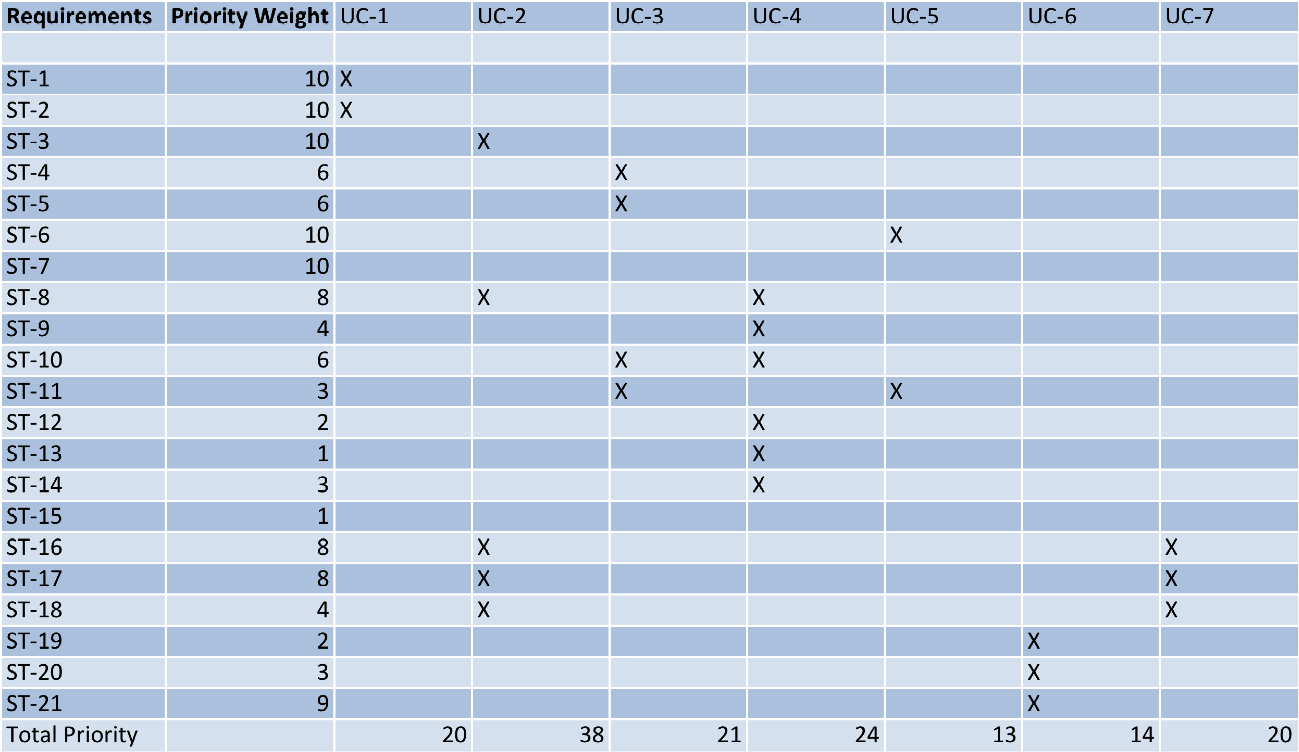
\includegraphics[width=5.5in]{./img/traceability.png}
\caption{The traceability matrix for the given use cases.}
\end{figure}

